\chapter{The Central Limit Theorem and Normal Approximation}

The normal distribution is important not only as a model for measurements but because
sums and averages of many independent random variables are approximately normal, almost
regardless of the distribution of the individual terms. This chapter makes that precise.

\section{Linear combinations of independent normals}

\begin{theorem}
If $X_1,\dots,X_n$ are independent with $X_i\sim\Norm(\mu_i,\sigma_i^2)$, and
$a_1,\dots,a_n, b$ are constants, then
\[
  \sum_{i=1}^n a_iX_i + b \sim \Norm\Big(\sum a_i\mu_i + b,\ \sum a_i^2\sigma_i^2\Big).
\]
\end{theorem}

The mean and variance follow from Chapter 8; the fact that the result is \emph{exactly}
normal is proved most easily with moment generating functions (Chapter 10).

\begin{corollary}
If $X_1,\dots,X_n$ are independent $\Norm(\mu,\sigma^2)$, then
\[
  \sum_{i=1}^n X_i\sim\Norm(n\mu, n\sigma^2) \qquad\text{and}\qquad
  \bar X\sim\Norm\left(\mu, \frac{\sigma^2}{n}\right).
\]
\end{corollary}

\begin{example}[Sum and difference]
Let $X\sim\Norm(5,4)$ and $Y\sim\Norm(3,9)$ be independent.
\begin{itemize}
  \item $X + Y\sim\Norm(8, 13)$, so
        $P(X+Y>10) = P\left(Z > \frac{2}{\sqrt{13}}\right) = P(Z > 0.55)
        = 1 - 0.70884 \approx 0.2912$.
  \item $X - Y\sim\Norm(2, 13)$ (variances add!), so
        $P(X > Y) = P(X - Y > 0) = P(Z > -2/\sqrt{13}) = P(Z > -0.55) = 0.70884$.
\end{itemize}
\end{example}

\begin{example}[Sample mean]
Package weights are $\Norm(50, 10^2)$ independently. For a sample of $n=25$,
$\bar X\sim\Norm(50, 100/25) = \Norm(50, 2^2)$, so
\[
  P(\bar X > 53) = P\left(Z > \frac{53-50}{2}\right) = P(Z > 1.5) = 1 - 0.93319 = 0.0668.
\]
A single package exceeds $53$ with probability $P(Z > 0.3) \approx 0.382$: averages are
much less variable than individual observations.
\end{example}

\begin{center}
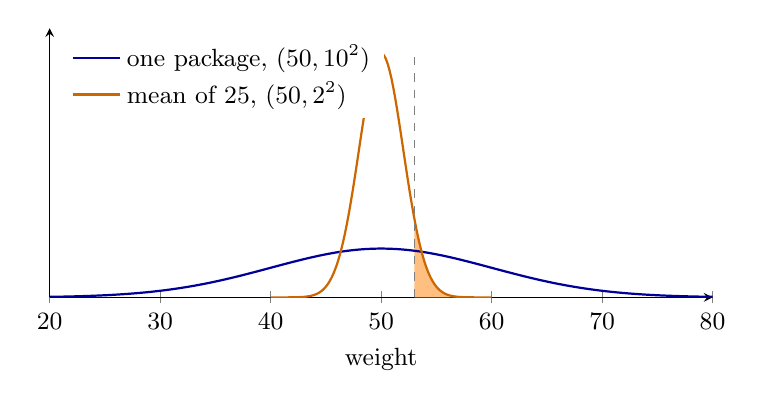
\begin{tikzpicture}
\begin{axis}[width=10cm, height=5cm, xmin=20, xmax=80, ymin=0, ymax=0.22, xlabel={weight},
    ytick=\empty, tick label style={font=\small}, label style={font=\small}, axis lines=left, scaled y ticks=false, yticklabel style={/pgf/number format/fixed}, samples=120, legend style={font=\small, draw=none, at={(0.02,0.98)}, anchor=north west}, legend cell align=left]
  \addplot[draw=none, fill=orange!50, domain=53:60, forget plot] {exp(-(x-50)^2/8)/(2*sqrt(2*pi))} \closedcycle;
  \addplot[thick, blue!60!black, domain=20:80] {exp(-(x-50)^2/200)/(10*sqrt(2*pi))};
  \addplot[thick, orange!80!black, domain=40:60] {exp(-(x-50)^2/8)/(2*sqrt(2*pi))};
  \draw[dashed, gray] (axis cs:53,0) -- (axis cs:53,0.2);
  \legend{{one package, $\Norm(50,10^2)$}, {mean of 25, $\Norm(50,2^2)$}}
\end{axis}
\end{tikzpicture}
\end{center}
The shaded area beyond $53$ under the narrow curve is $0.0668$; under the wide curve the
corresponding area would be $0.382$.

\begin{example}[Two independent copies vs.\ doubling]
If $X_1, X_2\sim\Norm(10, 4)$ independently, then $X_1+X_2\sim\Norm(20, 8)$ while
$2X_1\sim\Norm(20, 16)$. The sum of two independent copies is less spread out because
large and small values partially cancel.
\end{example}

\section{The central limit theorem}

\begin{theorem}[Central limit theorem (CLT)]
Let $X_1, X_2, \dots$ be independent and identically distributed with mean $\mu$ and
finite variance $\sigma^2$. Let $S_n = X_1+\cdots+X_n$ and $\bar X_n = S_n/n$. Then for
every real $z$,
\[
  \lim_{n\to\infty}P\left(\frac{S_n - n\mu}{\sigma\sqrt n}\le z\right) =
  \lim_{n\to\infty}P\left(\frac{\bar X_n - \mu}{\sigma/\sqrt n}\le z\right) = \Phi(z).
\]
\end{theorem}

In practice: for large $n$,
\[
  S_n\ \dot\sim\ \Norm(n\mu, n\sigma^2), \qquad \bar X_n\ \dot\sim\ \Norm\left(\mu,
  \frac{\sigma^2}{n}\right),
\]
where $\dot\sim$ means ``approximately distributed as''. How large $n$ must be depends on
the shape of the distribution of $X_i$: for symmetric distributions $n$ around $10$ is
often enough, while for very skewed ones (such as the exponential) $n$ of $30$ or more may
be needed. A proof sketch using moment generating functions is given in Chapter 10.

\begin{important}[What the CLT does and does not say]
The CLT is about the distribution of the \emph{sum or average}, not about the individual
$X_i$. Taking more observations does not make the data themselves look normal. The mean
and variance of $S_n$ ($n\mu$ and $n\sigma^2$) are exact for any $n$; only the normal
shape is an approximation.
\end{important}


\begin{center}
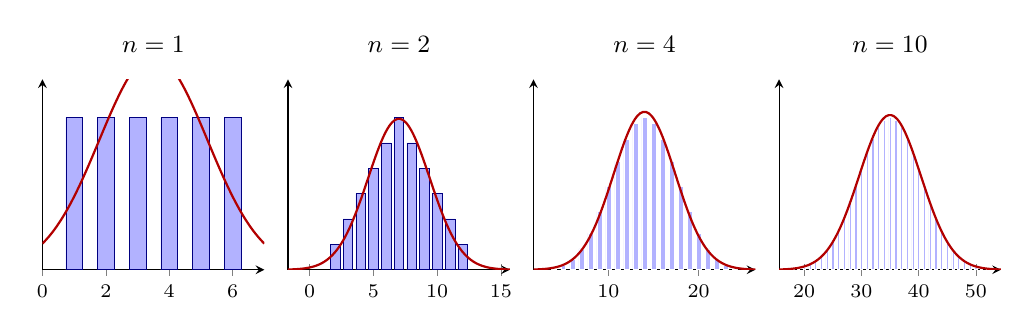
\begin{tikzpicture}
\begin{axis}[name=c0, width=4.4cm, height=4cm, ybar, bar width=6pt, bar shift=0pt,
    xmin=0.0, xmax=7.0, ymin=0, ymax=0.2083, ytick=\empty, title={$n = 1$},
    title style={font=\small}, tick label style={font=\scriptsize}, axis lines=left]
  \addplot[fill=blue!30, draw=blue!50!black, line width=0.2pt] coordinates {(1,0.16667) (2,0.16667) (3,0.16667) (4,0.16667) (5,0.16667) (6,0.16667)};
  \addplot[thick, red!70!black, domain=0.0:7.0, samples=80, smooth] {exp(-(x-3.5)^2/(2*2.9167))/sqrt(2*pi*2.9167)};
\end{axis}
\begin{axis}[name=c1, at={(c0.east)}, anchor=west, xshift=0.3cm, width=4.4cm, height=4cm, ybar, bar width=3.5pt, bar shift=0pt,
    xmin=-1.7, xmax=15.7, ymin=0, ymax=0.2083, ytick=\empty, title={$n = 2$},
    title style={font=\small}, tick label style={font=\scriptsize}, axis lines=left]
  \addplot[fill=blue!30, draw=blue!50!black, line width=0.2pt] coordinates {(2,0.02778) (3,0.05556) (4,0.08333) (5,0.11111) (6,0.13889) (7,0.16667) (8,0.13889) (9,0.11111) (10,0.08333) (11,0.05556) (12,0.02778)};
  \addplot[thick, red!70!black, domain=-1.7:15.7, samples=80, smooth] {exp(-(x-7.0)^2/(2*5.8333))/sqrt(2*pi*5.8333)};
\end{axis}
\begin{axis}[name=c2, at={(c1.east)}, anchor=west, xshift=0.3cm, width=4.4cm, height=4cm, ybar, bar width=1.8pt, bar shift=0pt,
    xmin=1.7, xmax=26.3, ymin=0, ymax=0.1408, ytick=\empty, title={$n = 4$},
    title style={font=\small}, tick label style={font=\scriptsize}, axis lines=left]
  \addplot[fill=blue!30, draw=white, line width=0.2pt] coordinates {(4,0.00077) (5,0.00309) (6,0.00772) (7,0.01543) (8,0.02701) (9,0.04321) (10,0.06173) (11,0.08025) (12,0.09645) (13,0.10802) (14,0.11265) (15,0.10802) (16,0.09645) (17,0.08025) (18,0.06173) (19,0.04321) (20,0.02701) (21,0.01543) (22,0.00772) (23,0.00309) (24,0.00077)};
  \addplot[thick, red!70!black, domain=1.7:26.3, samples=80, smooth] {exp(-(x-14.0)^2/(2*11.6667))/sqrt(2*pi*11.6667)};
\end{axis}
\begin{axis}[name=c3, at={(c2.east)}, anchor=west, xshift=0.3cm, width=4.4cm, height=4cm, ybar, bar width=0.8pt, bar shift=0pt,
    xmin=15.6, xmax=54.4, ymin=0, ymax=0.0909, ytick=\empty, title={$n = 10$},
    title style={font=\small}, tick label style={font=\scriptsize}, axis lines=left]
  \addplot[fill=blue!30, draw=white, line width=0.2pt] coordinates {(16,0.00008) (17,0.00019) (18,0.00039) (19,0.00077) (20,0.00141) (21,0.00245) (22,0.00403) (23,0.00634) (24,0.00954) (25,0.01375) (26,0.01904) (27,0.02539) (28,0.03262) (29,0.04046) (30,0.04846) (31,0.05612) (32,0.06287) (33,0.06816) (34,0.07153) (35,0.07269) (36,0.07153) (37,0.06816) (38,0.06287) (39,0.05612) (40,0.04846) (41,0.04046) (42,0.03262) (43,0.02539) (44,0.01904) (45,0.01375) (46,0.00954) (47,0.00634) (48,0.00403) (49,0.00245) (50,0.00141) (51,0.00077) (52,0.00039) (53,0.00019) (54,0.00008)};
  \addplot[thick, red!70!black, domain=15.6:54.4, samples=80, smooth] {exp(-(x-35.0)^2/(2*29.1667))/sqrt(2*pi*29.1667)};
\end{axis}
\end{tikzpicture}
\end{center}
The exact p.f.\ of the total of $n$ dice (bars) against the normal curve with the same mean
$3.5n$ and variance $35n/12$: the flat single-die distribution becomes a triangle at $n=2$
and is already very close to normal at $n=4$.

\begin{example}[Sum of dice]
A fair die is rolled $100$ times. Each roll has $\mu = 3.5$ and $\sigma^2 = 35/12$, so the
total $S$ has mean $350$ and variance $100\cdot 35/12 \approx 291.67$ (standard deviation
$17.08$). Since $S$ is integer-valued we use a continuity correction (see below):
\[
  P(S\le 370) = P(S\le 370.5) \approx P\left(Z\le\frac{20.5}{17.08}\right) =
  P(Z\le 1.20) = 0.8849.
\]
\end{example}

\begin{example}[Light bulbs]
Bulb lifetimes are independent $\Exp(\theta = 100)$ hours (mean $100$, standard deviation
$100$). Fifty bulbs are used one after another. The total lifetime $T$ has mean $5000$ and
standard deviation $100\sqrt{50} \approx 707.1$, so
\[
  P(T > 5500) \approx P\left(Z > \frac{500}{707.1}\right) = P(Z > 0.71) = 1 - 0.76115
  \approx 0.2389.
\]
(No continuity correction: $T$ is continuous.)
\end{example}

\begin{example}[Choosing a sample size]
Measurements have standard deviation $\sigma = 2$. How large must $n$ be so that the
sample mean is within $0.5$ of $\mu$ with probability at least $0.95$? By the CLT,
\[
  P(\abs{\bar X - \mu} < 0.5) \approx P\left(\abs{Z} < \frac{0.5\sqrt n}{2}\right) \ge 0.95
  \iff \frac{0.5\sqrt n}{2}\ge 1.96 \iff n\ge\left(\frac{1.96\cdot 2}{0.5}\right)^2 = 61.47.
\]
So $n = 62$ suffices.
\end{example}

\section{Normal approximation to the binomial and Poisson}

\begin{theorem}[De Moivre--Laplace]
If $X\sim\Bin(n,p)$, then for large $n$,
\[
  X\ \dot\sim\ \Norm(np, np(1-p)).
\]
\end{theorem}

\begin{proof}
$X = I_1 + \dots + I_n$ is a sum of independent, identically distributed indicators with
mean $p$ and variance $p(1-p)$; apply the CLT.
\end{proof}

A common rule of thumb is that the approximation is good when $np\ge5$ and
$n(1-p)\ge5$. (If $p$ is small and $np$ is small, the Poisson approximation of Chapter 5 is
better.)

\begin{theorem}[Normal approximation to the Poisson]
If $X\sim\Poi(\mu)$, then for large $\mu$,
\[
  X\ \dot\sim\ \Norm(\mu,\mu).
\]
\end{theorem}

\begin{proof}
For integer $\mu = n$, $X$ has the same distribution as a sum of $n$ independent
$\Poi(1)$ r.v.s (Chapter 8), so the CLT applies; the general case is similar.
\end{proof}

\subsection{The continuity correction}

A discrete r.v.\ puts all its probability on integers, while the normal spreads it
continuously. Think of $P(X = k)$ as the area of a histogram bar over $[k-0.5, k+0.5]$.

\begin{important}[Continuity correction for integer-valued $X$]
\begin{center}
\begin{tabular}{ll}
\toprule
Discrete event & Use in the normal approximation \\
\midrule
$P(X\le k)$ & $P(X\le k+0.5)$ \\
$P(X < k) = P(X\le k-1)$ & $P(X\le k-0.5)$ \\
$P(X\ge k)$ & $P(X\ge k-0.5)$ \\
$P(X = k)$ & $P(k-0.5\le X\le k+0.5)$ \\
$P(a\le X\le b)$ & $P(a-0.5\le X\le b+0.5)$ \\
\bottomrule
\end{tabular}
\end{center}
Rewrite strict inequalities as non-strict ones first.
\end{important}

\begin{example}[Coin tosses]
A fair coin is tossed $100$ times; $X\sim\Bin(100, 0.5)$ with mean $50$ and standard
deviation $\sqrt{25} = 5$.
\begin{itemize}
  \item $P(X\le55)\approx P\left(Z\le\frac{55.5-50}{5}\right) = \Phi(1.1) = 0.8643$.
        The exact binomial value is $0.8644$. Without the correction we would get
        $\Phi(1.0) = 0.8413$, noticeably worse.
  \item $P(X = 50) \approx P(49.5\le X\le 50.5) = P(-0.1\le Z\le0.1) = 2(0.53983) - 1
        = 0.0797$; the exact value is $\binom{100}{50}/2^{100}\approx 0.0796$. (Without
        the correction we would get $0$!)
\end{itemize}
\end{example}

\begin{example}[An interval]
$X\sim\Bin(50, 0.4)$ has mean $20$ and variance $12$ (standard deviation $3.464$). Then
\begin{align*}
  P(18\le X\le 24) &\approx P\left(\frac{17.5-20}{3.464}\le Z\le\frac{24.5-20}{3.464}\right)
  = P(-0.72\le Z\le 1.30) \\
  &= 0.90320 - (1-0.76424) = 0.6674.
\end{align*}
The exact binomial probability is $0.6653$.
\end{example}

\begin{center}
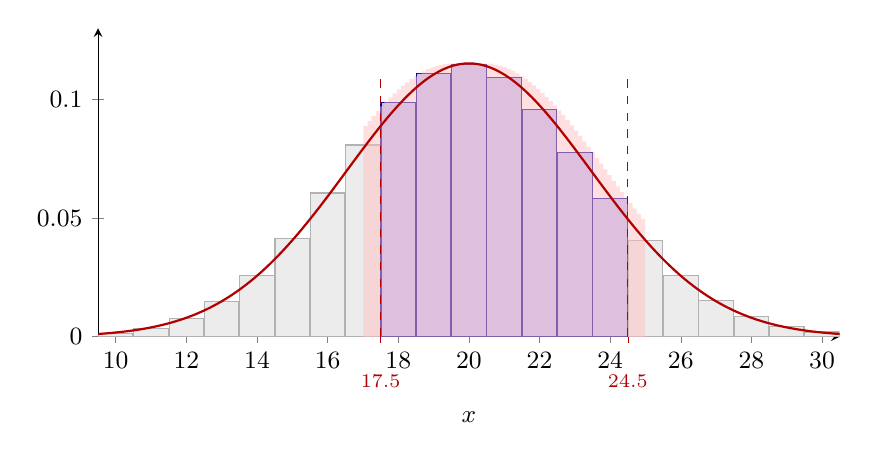
\begin{tikzpicture}
\begin{axis}[width=11cm, height=5.5cm, ybar, bar width=12.5pt, bar shift=0pt, xmin=9.5, xmax=30.5,
    ymin=0, ymax=0.13, xtick={10,12,...,30}, extra x ticks={17.5,24.5},
    extra x tick style={tick label style={font=\scriptsize, text=red!70!black, yshift=-8pt}, tick style={red!70!black}},
    xlabel={$x$}, tick label style={font=\small}, label style={font=\small}, axis lines=left, scaled y ticks=false, yticklabel style={/pgf/number format/fixed}]
  \addplot[fill=gray!15, draw=gray!60] coordinates {(10,0.00144) (11,0.00349) (12,0.00756) (13,0.01474) (14,0.02597) (15,0.04155) (16,0.06059) (17,0.08079) (25,0.04046) (26,0.02594) (27,0.01537) (28,0.00842) (29,0.00426) (30,0.00199)};
  \addplot[fill=blue!25, draw=blue!60!black] coordinates {(18,0.09874) (19,0.11086) (20,0.11456) (21,0.10910) (22,0.09588) (23,0.07781) (24,0.05836)};
  \addplot[draw=none, fill=red!25, fill opacity=0.5, domain=17.5:24.5, samples=60] {exp(-(x-20)^2/24)/sqrt(24*pi)} \closedcycle;
  \addplot[thick, red!70!black, domain=9.5:30.5, samples=100, smooth] {exp(-(x-20)^2/24)/sqrt(24*pi)};
  \draw[red!70!black, dashed] (axis cs:17.5,0) -- (axis cs:17.5,0.11);
  \draw[red!70!black, dashed] (axis cs:24.5,0) -- (axis cs:24.5,0.11);
\end{axis}
\end{tikzpicture}
\end{center}
The blue bars are $P(X = 18), \dots, P(X = 24)$; each bar covers $[k-0.5, k+0.5]$, so the
matching area under the $\Norm(20,12)$ curve runs from $17.5$ to $24.5$, not from $18$ to $24$.

\begin{example}[Poisson]
Customers arrive at a store according to a Poisson process, averaging $25$ per hour. Let
$X\sim\Poi(25)$ be the number in a given hour. Then
\[
  P(X\ge 30) = P(X\ge 29.5) \approx P\left(Z\ge\frac{29.5-25}{5}\right) = P(Z\ge 0.9)
  = 1 - 0.81594 = 0.1841,
\]
compared with the exact value $0.1821$.
\end{example}

\section{Summary}

\begin{itemize}
  \item Linear combinations of independent normals are exactly normal, with
        mean $\sum a_i\mu_i + b$ and variance $\sum a_i^2\sigma_i^2$.
  \item CLT: for i.i.d.\ $X_i$ with mean $\mu$ and variance $\sigma^2$,
        $S_n\ \dot\sim\ \Norm(n\mu, n\sigma^2)$ and $\bar X\ \dot\sim\ \Norm(\mu,\sigma^2/n)$.
  \item $\Bin(n,p)\ \dot\sim\ \Norm(np, np(1-p))$ when $np$, $n(1-p)\ge 5$;
        $\Poi(\mu)\ \dot\sim\ \Norm(\mu,\mu)$ for large $\mu$.
  \item Use the $\pm0.5$ continuity correction when approximating an integer-valued r.v.
\end{itemize}
